\documentclass{standalone}
\usepackage{tikz}
\usepackage{ctex,siunitx}
\usepackage{tkz-euclide}
\usepackage{amsmath}
\usetikzlibrary{patterns, calc}
\usetikzlibrary {decorations.pathmorphing, decorations.pathreplacing, decorations.shapes,}
\begin{document}
\small
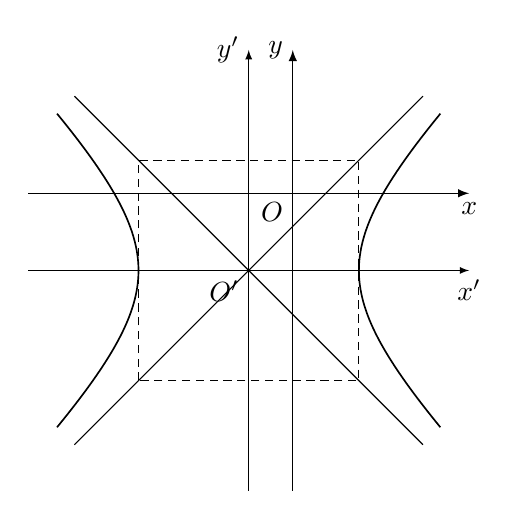
\begin{tikzpicture}[>=latex,scale=0.14,samples=200]
  \draw[very thin,->](-20,0)--(20,0)node[below]{$x'$};
  \draw[very thin,->](0,-20)--(0,20)node[left]{$y'$};
  \draw[thin,->](-20,7)--(20,7)node[below]{$x$};
  \draw[thin,->](4,-20)--(4,20)node[left]{$y$};
  \tkzDefPoints{0/0/O',4/7/O}
  \tkzLabelPoints[below left](O,O')
  \draw[thin,densely dashed](-10,-10)rectangle(10,10);
  \begin{scope}[rotate=-45,scale=2.236]
    \draw(-10,0)--(10,0)(0,-10)--(0,10);
    \draw [semithick,domain=1:10]  plot (\x,{10/\x});
    \draw [semithick,domain=-1:-10]  plot (\x,{10/\x});
  \end{scope}
\end{tikzpicture}
\end{document}